\documentclass{article}

% Set page size and margins
% Replace `letterpaper' with `a4paper' for UK/EU standard size
\usepackage[letterpaper,top=2cm,bottom=2cm,left=3cm,right=3cm,marginparwidth=1.75cm]{geometry}
\usepackage[spanish]{babel}
\usepackage{url}
\usepackage{hyperref}
\usepackage{csquotes}
\usepackage{amsmath}
\usepackage{amssymb}
\usepackage{graphicx}
\usepackage{listings}
\usepackage{xcolor}
\usepackage{setspace}
\usepackage{float}

\graphicspath{ {assets/} }

%Code colors:
\definecolor{codegreen}{rgb}{0,0.6,0}
\definecolor{codegray}{rgb}{0.5,0.5,0.5}
\definecolor{codepurple}{rgb}{0.58,0,0.82}
\definecolor{backcolour}{rgb}{0.95,0.95,0.92}
\doublespacing

\lstdefinestyle{mystyle}{
    backgroundcolor=\color{backcolour},
    commentstyle=\color{codegreen},
    keywordstyle=\color{magenta},
    numberstyle=\tiny\color{codegray},
    stringstyle=\color{codepurple},
    basicstyle=\ttfamily\footnotesize,
    breakatwhitespace=false,
    breaklines=false,
    captionpos=b,
    keepspaces=true,
    numbers=left,
    numbersep=5pt,
    showstringspaces=false,
    showlines=false,
    showtabs=false,
    tabsize=2
}

\lstset{style=mystyle}

\NewDocumentCommand{\codeword}{v}{%
    \texttt{\textcolor{black}{#1}}%
}

\begin{document}

    \begin{titlepage}
        \centering
        {
\includegraphics[width=0.5\textwidth]{assets/logo2}\par}
        {\bfseries\LARGE Universidad Católica del Uruguay \par}
        \vspace{0.3cm}
        {\scshape\Large Facultad de Ingeniería \par}
        \vspace{0.3cm}
        {\scshape\Huge Proyecto - Polinomios de Taylor\par}
        \vspace{1cm}
        {\Large Cálculo Aplicado \par}
        {\Large Profesores: Maglis Mujica y Martín Perciante \par}
        \vfill
        {\Large Autores: \par}
        {\Large Luis Balduini (4.001.184-9)\\Leandro Casaretto (5.400.457-7)\\Juan Manuel Pérez (4.673.899-0) \par}
        \vfill
        {\Large \today \par}
    \end{titlepage}

    \section{Introducción}\label{sec:intro}
El presente informe aborda el uso del \textbf{polinomio de Taylor} como
herramienta para aproximar modelos físicos y simplificar la resolución de
problemas que, de otro modo, requerirían técnicas analíticas avanzadas.Se consideran dos situaciones independientes:

\begin{itemize}
\item \textbf{Parte 1:} la variación de la aceleración gravitatoria con la
distancia al centro terrestre, basada en la ley de gravitación universal.
\item \textbf{Parte 2:} la caída libre vertical con \emph{rozamiento lineal}
(fuerza de arrastre proporcional a la velocidad).
\end{itemize}

Ambos casos comparten el objetivo de responder: \emph{¿en qué régimen es
válido reemplazar la función exacta por un polinomio de baja orden y qué
error se comete?}

% --------------------------------------------------------------------
\section{Marco Teórico: Polinomios de Taylor}

\subsection{Definición y Motivación}
Sea $f$ una función real de variable real suficientemente diferenciable en un entorno de un punto $a$. El polinomio de Taylor de grado $n$ de la función $f$ centrado en $a$ se define como:
\[
P_n(f,a;x) = \sum_{k=0}^{n} \frac{f^{(k)}(a)}{k!}(x - a)^k.
\]
Este polinomio ofrece una aproximación de $f$ cerca de $x = a$, aprovechando la información de las derivadas de orden inferior.

\subsection{Teorema de Taylor con Resto}
El Teorema de Taylor establece que, si $f$ es de clase $C^{n+1}$ en un intervalo que contiene a $a$ y $x$, existe un punto $\xi$ entre $a$ y $x$ tal que:
\[
f(x) = P_n(f,a;x) + R_{n+1}(x),
\]
donde el resto en forma de Lagrange está dado por:
\[
R_{n+1}(x) = \frac{f^{(n+1)}(\xi)}{(n+1)!}(x - a)^{n+1}.
\]
Esta expresión cuantifica el error de aproximación cuando se utiliza el polinomio de grado $n$.

\subsection{Propiedades Fundamentales}
\begin{itemize}
  \item Para $n=0$, $P_0(f,a;x)=f(a)$; la aproximación es constante.
  \item Para $n=1$, $P_1(f,a;x)=f(a) + f'(a)(x-a)$; tangente lineal.
  \item Si $f$ es polinómica de grado $\le n$, entonces $R_{n+1}(x)=0$; la aproximación es exacta.
  \item El polinomio de Taylor converge a $f$ cuando $n\to\infty$ si $\lim_{n\to\infty} R_{n+1}(x) = 0$ para $x$ en el intervalo.
\end{itemize}

% --------------------------------------------------------------------
\section{Desarrollo}\label{sec:desarrollo}
A continuación se presentan los desarrollos planteados en el informe, divididos en dos partes según los problemas planteados.

\subsection{Modelo de Gravitación Universal}

Se considera la aceleración gravitatoria como una función de la distancia $r$ al centro de la Tierra, dada por:

\[
\vec{a}(r) = f(r) = -\frac{GM}{r^2}
\]

\subsubsection*{Valores base utilizados para los cálculos}

\begin{itemize}
    \item $G = 6{,}67430 \times 10^{-11} \; \mathrm{Nm^2/kg^2}$
    \item $M = 5{,}972 \times 10^{24} \; \mathrm{kg}$
    \item $R_T = 6{,}371 \times 10^{6} \; \mathrm{m}$ \hfill (Radio de la Tierra)
    \item $GM = 3{,}986004418 \times 10^{14} \; \mathrm{m^3/s^2}$
\end{itemize}

\subsubsection{Desarrollo con Polinomio de Taylor de orden 1}

Se toma la función:

\[
f(r) = -\frac{GM}{r^2}
\quad \text{con} \quad r_0 = R_T
\]

El desarrollo de Taylor de orden 1 alrededor de $r_0$ es:

\[
f(r) \approx f(r_0) + f'(r_0)(r - r_0)
\]

\[
f(R_T) = -\frac{GM}{R_T^2}
\]

Derivamos la función original:

\[
f(r) = -\frac{GM}{r^2}
\quad \Rightarrow \quad
f'(r) = \frac{d}{dr} \left( -GM \cdot r^{-2} \right) = 2GM \cdot r^{-3} = \frac{2GM}{r^3}
\]

Evaluando la derivada en $r = R_T$:

\[
f'(R_T) = \frac{2GM}{R_T^3}
\]

Entonces, el polinomio de Taylor de orden 1 alrededor de $R_T$ es:

\[
P_1(r) = f(R_T) + f'(R_T)(r - R_T) = -\frac{GM}{R_T^2} + \frac{2GM}{R_T^3}(r - R_T)
\]

\subsubsection{Evaluación en RT+h con h = 8849 m}

Dado que $r = R_T + h$, entonces:

\[
f(R_T + h) = -\frac{GM}{(R_T + h)^2}
\]

Ya habíamos calculado:

\[
f(R_T) = -\frac{GM}{R_T^2} = -\frac{3{,}986004418 \times 10^{14}\ \text{m}^3/\text{s}^2}{(6{,}371 \times 10^6\ \text{m})^2} = -9.82025\ \text{m/s}^2
\]

\[
f(R_T + h) = -\frac{3{,}986004418 \times 10^{14}\ \text{m}^3/\text{s}^2}{(6{,}371 \times 10^6\ \text{m} + 8849\ \text{m})^2} = -9.79303\ \text{m/s}^2
\]

Calculamos el cambio relativo:

\[
\Delta_{\text{rel}} = \frac{f(R_T + h) - f(R_T)}{f(R_T)} = \frac{-GM[(R_T + h)^{-2} - R_T^{-2}]}{-GM \cdot R_T^{-2}} = \left( \frac{1}{(1 + \frac{h}{R_T})^2} \right) - 1
\]

\[
\frac{h}{R_T} = \frac{8849}{6{,}371{,}000} = 1.388 \times 10^{-3}
\quad \Rightarrow \quad
\Delta_{\text{rel}} = (1 + 1.388 \times 10^{-3})^{-2} - 1 = -2.772 \times 10^{-3}
\]

\[
\text{Equivalente a } 0.277\%
\]

\noindent
Este pequeño cambio sugiere que, para variaciones de altura como $h = 8849\ \text{m}$, el valor de $g$ puede considerarse constante sin pérdida significativa de precisión.

\vspace{0.5em}
\noindent
Podemos también aproximar $f(R_T + h)$ usando el polinomio de Taylor de orden 1 calculado previamente:

\[
P_1(R_T + h) = -\frac{GM}{R_T^2} + \frac{2GM}{R_T^3} \cdot h
\]

\subsubsection{Polinomio de Taylor de orden 2 en RT + h}

La función que estamos considerando es:
\[
f(r) = -\frac{GM}{r^2}
\]

Ya se obtuvieron las siguientes derivadas:
\[
f'(r) = \frac{2GM}{r^3}, \qquad f''(r) = -\frac{6GM}{r^4}
\]

Por lo tanto, el polinomio de Taylor de orden 2 alrededor de $r_0 = R_T$ es:

\[
P_2(R_T + h) = f(R_T) + f'(R_T) \cdot h + \frac{1}{2} f''(R_T) \cdot h^2
\]

Sustituyendo los valores conocidos:
\[
f(R_T) = -\frac{GM}{R_T^2}, \quad
f'(R_T) = \frac{2GM}{R_T^3}, \quad
f''(R_T) = -\frac{6GM}{R_T^4}
\]

\[
P_2(R_T + h) = -\frac{GM}{R_T^2} + \frac{2GM}{R_T^3} \cdot h - \frac{1}{2} \cdot \frac{6GM}{R_T^4} \cdot h^2
\]

\[
\Rightarrow P_2(R_T + h) = -\frac{GM}{R_T^2} + \frac{2GM}{R_T^3} \cdot h - \frac{3GM}{R_T^4} \cdot h^2
\]

Al momento de realizar las operaciones, se obtiene:
\[
P_2(R_T + h) = -9.82025 + 0.02727 \cdot h - 0.00000569 \cdot h^2 = -9.79304 \text{ m/s}^2
\]

\noindent \textbf{Comparación:}\\
Valor exacto: $-9.79303\ \text{m/s}^2$ \\
Polinomio de Taylor de orden 2: $-9.79304\ \text{m/s}^2$ \\


Este polinomio permite una aproximación más precisa de la aceleración gravitatoria a una altura $h$ sobre la superficie terrestre, considerando también el efecto cuadrático del cambio de altura.

\subsubsection{Gráfica de r0 = RT y polinomio de Taylor de orden 2}

Para analizar el comportamiento del polinomio de Taylor de orden 2 con respecto a la función original de aceleración gravitatoria, se realizó una gráfica que compara ambas expresiones en el rango $[R_T, R_T + 20\,000]$ m, es decir, desde la superficie de la Tierra hasta 20 km de altitud.

\begin{itemize}
    \item En azul se presenta la función original: $f(r) = -\dfrac{GM}{r^2}$.
    \item En rojo punteado, el polinomio de Taylor de orden 2, centrado en $R_T$.
    \item Se incluye una línea vertical verde indicando la altura del Monte Everest ($8849$ m).
\end{itemize}

Como se puede observar, el polinomio de Taylor aproxima de forma muy precisa a la función original en el entorno inmediato de $R_T$. A medida que la altura se incrementa, la diferencia se vuelve levemente más significativa, aunque aún menor al 1\%, validando el uso del polinomio para pequeñas alturas.

\begin{figure}[H]
    \centering
    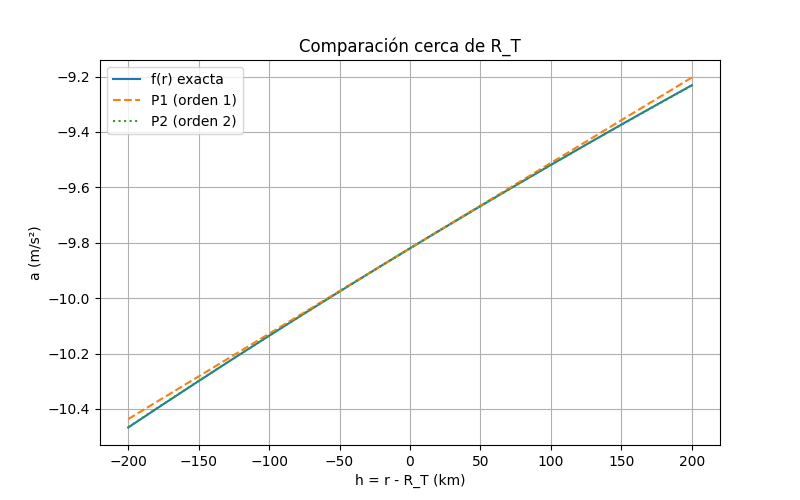
\includegraphics[width=1\textwidth]{assets/taylor_vs_gravedad.png}
    \caption{Gráfica de $r_0 = R_T$ y polinomio de Taylor de orden 2}
\end{figure}

\subsubsection{¿Cuánto debe alejarse un cuerpo para que g sea 1\% menor?}

Queremos encontrar la distancia $r$ tal que la aceleración gravitatoria disminuya un 1\% respecto a la que se experimenta en la superficie terrestre. Es decir:

\[
|f(R_T)| = \frac{GM}{R_T^2}, \quad \text{y queremos:} \quad \frac{GM}{r^2} = 0{,}99 \cdot \frac{GM}{R_T^2}
\]

Cancelando $GM$ en ambos lados de la ecuación:

\[
\frac{1}{r^2} = 0{,}99 \cdot \frac{1}{R_T^2} \quad \Rightarrow \quad r^2 = \frac{R_T^2}{0{,}99}
\]

\[
r = \frac{R_T}{\sqrt{0{,}99}} \approx 6\,403\,095\,\text{m}
\]

\[
h = r - R_T = 6\,403\,095 - 6\,371\,000 = 32\,096\,\text{m} \quad (\text{equivalente a } 32{,}1\,\text{km})
\]

\vspace{0.5em}

\textbf{Aproximación con el desarrollo de Taylor:}

Recordando que el cambio relativo en la aceleración se aproxima por:

\[
\Delta_{\text{rel}} \approx \frac{2h}{R_T} \quad \Rightarrow \quad h = \frac{\Delta_{\text{rel}} \cdot R_T}{2}
\]

Para $\Delta_{\text{rel}} = -0{,}01$:

\[
h \approx \frac{0{,}01 \cdot R_T}{2} = 0{,}005 \cdot R_T \approx 31\,855\,\text{m}
\]

\vspace{0.5em}

\textbf{Conclusión:} Se verifica que un cuerpo debe alejarse aproximadamente $32\,\text{km}$ de la superficie terrestre para que la aceleración gravitatoria sea un 1\% menor. Esta estimación es coherente tanto con el cálculo exacto como con la aproximación de Taylor.

\subsubsection{Radios 0,01 m y 0,02 m}

Analizamos la función de aceleración gravitatoria para radios extremadamente pequeños:

\[
f(r) = -\frac{GM}{r^2}
\]

Evaluando en $r = 0{,}01\,\text{m}$:

\[
f(0{,}01) = -\frac{GM}{(0{,}01)^2} = -\frac{GM}{1 \cdot 10^{-4}} = -GM \cdot 10^4
\]

Evaluando en $r = 0{,}02\,\text{m}$:

\[
f(0{,}02) = -\frac{GM}{(0{,}02)^2} = -\frac{GM}{4 \cdot 10^{-4}} = -\frac{GM \cdot 10^4}{4}
\]

\[
\Rightarrow \quad f(0{,}02) = \frac{1}{4} \cdot f(0{,}01)
\]

Se calcula la variación relativa de la aceleración gravitatoria al duplicar el radio desde $0{,}01\,\text{m}$ a $0{,}02\,\text{m}$:

\[
\Delta_{\text{rel}} = \frac{f(0{,}02) - f(0{,}01)}{f(0{,}01)} = \frac{\left(\frac{1}{4}f(0{,}01) - f(0{,}01)\right)}{f(0{,}01)} = -0{,}75
\]

\textbf{Interpretación:} La aceleración disminuye un $75\%$ al duplicar el radio.

\vspace{0.5cm}

\textbf{Desarrollo con polinomio de Taylor (orden 2) alrededor de $r_0 = 0{,}01\,\text{m}$}

\begin{align*}
f(r) &= -\frac{GM}{r^2} \\
f'(r) &= \frac{2GM}{r^3} \\
f''(r) &= -\frac{6GM}{r^4} \\
f^{(3)}(r) &= \frac{24GM}{r^5}
\end{align*}

Aplicando el polinomio de Taylor de segundo orden:

\[
P_2(r_0 + h) = f(r_0) + f'(r_0)h + \frac{f''(r_0)}{2}h^2
\]

Para $h = 0{,}01\,\text{m}$:

\[
P_2(2r_0) = -\frac{GM}{r_0^2} + \frac{2GM}{r_0^3} \cdot r_0 + \frac{-6GM}{2r_0^4} \cdot r_0^2
\]

\[
P_2(2r_0) = -\frac{GM}{r_0^2} + \frac{2GM}{r_0^2} - \frac{3GM}{r_0^2} = -\frac{2GM}{r_0^2}
\]

La aceleración predicha por Taylor de segundo orden a $r = 2r_0$ da una variación del $-0{,}25 \cdot f(r_0)$, es decir, una caída del $25\%$, lo cual difiere del valor real ($75\%$), evidenciando que el desarrollo de segundo orden no es suficiente para intervalos grandes.

Partimos del desarrollo de Taylor de orden 3 centrado en \( r_0 = 0{,}01\,\text{m} \):

\[
P_3(r_0 + h) = f(r_0) + f'(r_0) h + \frac{f''(r_0)}{2} h^2 + \frac{f^{(3)}(r_0)}{6} h^3
\]

Sabemos que:

\begin{align*}
f(r) &= -\frac{GM}{r^2} \\
f'(r) &= \frac{2GM}{r^3} \\
f''(r) &= -\frac{6GM}{r^4} \\
f^{(3)}(r) &= \frac{24GM}{r^5}
\end{align*}

Entonces, con \( h = r_0 \), se tiene:

\[
P_3(2r_0) = -\frac{GM}{r_0^2} + \frac{2GM}{r_0^2} - \frac{3GM}{r_0^2} + \frac{4GM}{r_0^2} = \frac{2GM}{r_0^2}
\]

\textbf{Interpretación:} El resultado obtenido al aplicar el polinomio de Taylor de orden 3 da un valor que cuadruplica el módulo del valor original de \( f(r_0) \), lo que indica que este desarrollo no es adecuado para estimar el valor de la función en un intervalo tan grande (de \( r_0 \) a \( 2r_0 \)). Este error significativo resalta que el desarrollo de Taylor tiene buena precisión únicamente en una cercanía al punto \( r_0 \).
También se observa que en el desarrollo de Taylor de orden 3, cambia de signo por lo cual se puede decir que en lugar de atraer, rechaza a los cuerpos, lo cual es físicamente incorrecto.

\subsubsection{Graficar r0 = 0.01 m para Polinomio de Taylor de orden 2 y 3}

\begin{figure}[H]
    \centering
    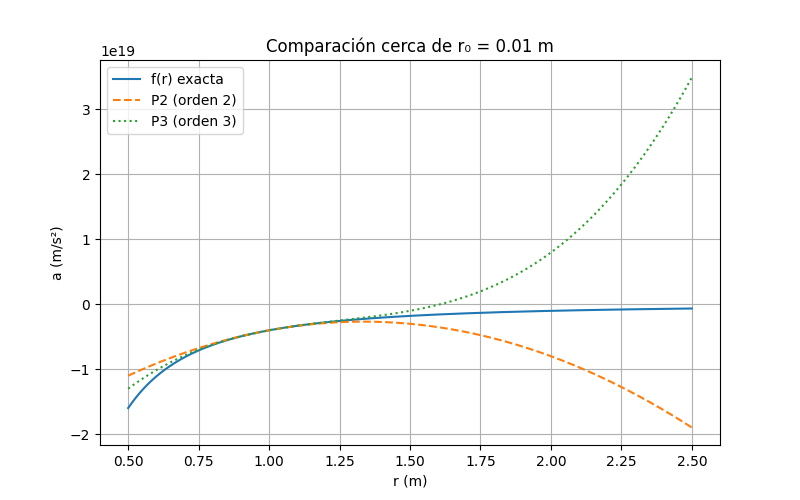
\includegraphics[width=1\textwidth]{assets/taylor_orden2y3.png}
    \caption{Gráfica de Taylor Orden 2 y 3 para $r_0 = 0.01$ m}
\end{figure}



\subsection{Caída con rozamiento lineal}
Ya se ha justificado el uso de un modelo con gravedad constante cerca de la superficie terrestre. Ahora se explorará el efecto del rozamiento del aire en el movimiento de un cuerpo en caída libre. 

Consideramos un cuerpo que cae verticalmente bajo la acción de la gravedad y una fuerza de rozamiento proporcional a su velocidad. Aplicando la segunda ley de Newton, la ecuación del movimiento es:

\[
m \frac{d^2y}{dt^2} = -b \frac{dy}{dt} - mg
\]

Definimos los parámetros:

\[
\gamma := \frac{b}{m}, \quad v_0 := \left.\frac{dy}{dt}\right|_{t=0}
\]

donde:
\begin{itemize}
\item \( \gamma \) representa la constante de rozamiento específica del cuerpo
\item \( v_0 \) es la velocidad inicial
\item \( y_0 \) es la posición inicial del cuerpo
\end{itemize}
La solución a esta ecuación diferencial, que representa la posición vertical del cuerpo en función del tiempo, se expresa como:

\[
y(t) = y_0 - \frac{g}{\gamma} t - \frac{1}{\gamma} \left( v_0 + \frac{g}{\gamma} \right) \left( e^{-\gamma t} - 1 \right)
\]

Este modelo supone que el movimiento es puramente vertical y no considera desplazamientos horizontales.

A continuación, se consideran tres valores distintos de \( \gamma \) para representar distintos tipos de cuerpos:

\begin{itemize}
    \item \( \gamma_h = 6.54\, \text{s}^{-1} \) (aproximación para una \textbf{hormiga})
    \item \( \gamma_p = 2.35 \times 10^{-1}\, \text{s}^{-1} \) (aproximación para una \textbf{persona})
    \item \( \gamma_a = 1.05 \times 10^{-2}\, \text{s}^{-1} \) (aproximación para un \textbf{auto})
\end{itemize}

\subsubsection{Comportamiento del desarrollo de Taylor de orden 2 alrededor de \( t = 0 \) y análisis para \( \gamma \) pequeño}

Se parte de la expresión para la posición con rozamiento:

\[
y(t) = y_0 - \frac{g}{\gamma} t - \frac{1}{\gamma} \left( v_0 + \frac{g}{\gamma} \right)(e^{-\gamma t} - 1)
\]

Calculamos las derivadas en \( t = 0 \):

\[
y'(t) = -\frac{g}{\gamma} + \left( v_0 + \frac{g}{\gamma} \right) e^{-\gamma t} \quad \Rightarrow \quad y'(0) = v_0
\]
\[
y''(t) = \gamma \left( v_0 + \frac{g}{\gamma} \right) e^{-\gamma t} \quad \Rightarrow \quad y''(0) = - (g + \gamma v_0)
\]

El polinomio de Taylor de orden 2 alrededor de \( t = 0 \) es:

\[
P_2(t) = y(0) + y'(0)t + \frac{1}{2} y''(0)t^2
\]

\noindent Comparando el modelo con aire y sin aire para \( v_0 \neq 0 \):

\[
\begin{array}{|c|c|}
\hline
\textbf{Sin aire} & \textbf{Con aire (Taylor O(2))} \\
\hline
v_0 \cdot t & v_0 \cdot t \\
-\frac{1}{2} g t^2 & -\frac{1}{2} (g + \gamma v_0) t^2 \\
\hline
\end{array}
\]

\paragraph{Análisis para \( \gamma \) pequeño:}

\begin{itemize}
    \item Si \( v_0 = 0 \Rightarrow y''(0) = -g \). El término de rozamiento no tiene efecto: se recupera el caso de caída libre.
    \item Si \( v_0 < 0 \) (movimiento descendente inicial) y \( \gamma > 0 \): 
    \[
    \gamma v_0 < 0 \Rightarrow |y''(0)| < g
    \]
    La aceleración disminuye: el aire frena la caída.
    \item Si \( v_0 > 0 \) (movimiento ascendente inicial): 
    \[
    y''(0) = -(g + \gamma v_0) < -g
    \]
    La aceleración aumenta en módulo, frenando más rápidamente la subida.
\end{itemize}

A continuación se presenta el gráfico que describe el comportamiento de las curvas para los distintos valores de \( \gamma \):
\begin{figure}[H]
    \centering
    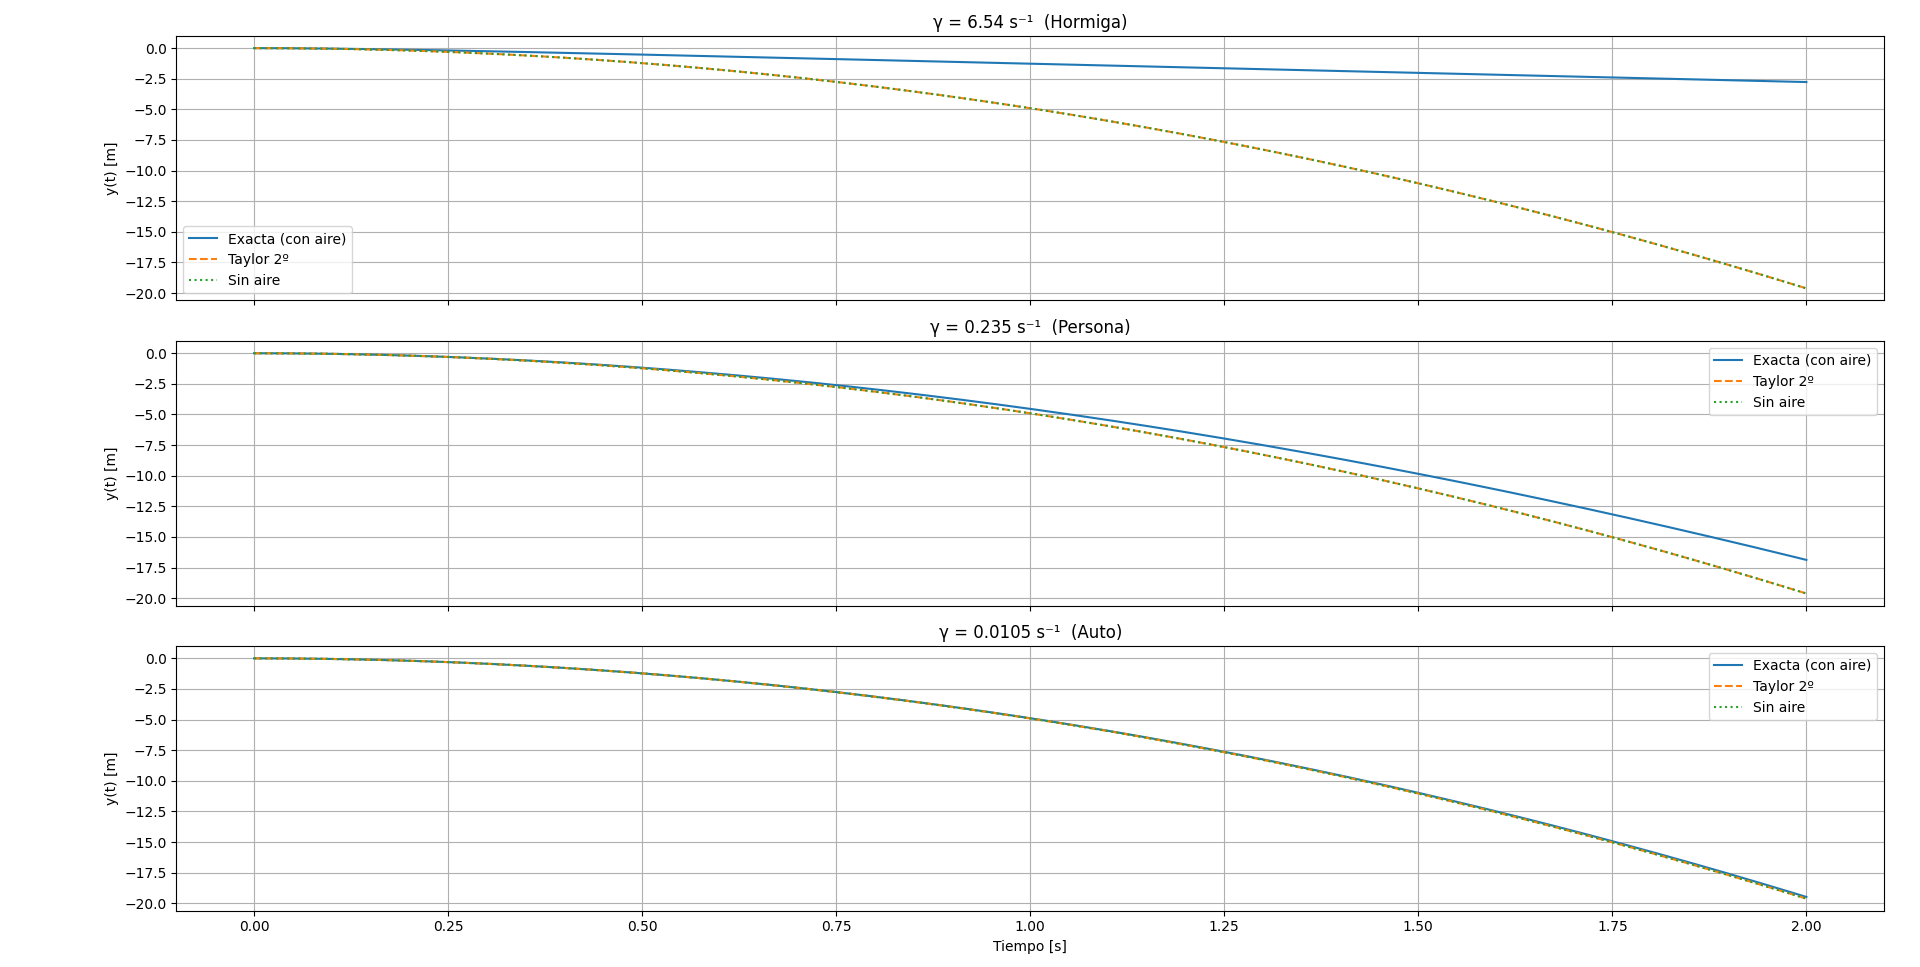
\includegraphics[width=1\textwidth]{assets/comparacion_curva_3modelos.png}
    \caption{Comparación de las curvas para los valores de \( \gamma \)}
\end{figure}

\paragraph{Conclusión:} 
Cuando \( \gamma \to 0 \), el término \( \gamma v_0 t^2 \) es de orden inferior y el movimiento se aproxima al caso sin aire. Por lo tanto, para valores muy pequeños de \( \gamma \), el polinomio de Taylor tiende al comportamiento de caída libre sin rozamiento.

\subsubsection{Evaluación de los tres modelos: con rozamiento, sin rozamiento y Taylor de orden 2}

Las funciones evaluadas son:
\begin{itemize}
    \item Con rozamiento: $y_{\text{cr}}(t) = y_0 - \frac{g}{\gamma}t - \frac{1}{\gamma}(v_0 + \frac{g}{\gamma})(e^{-\gamma t} - 1)$
    \item Sin rozamiento: $y_{\text{sr}}(t) = y_0 + v_0t - \frac{1}{2}gt^2$
    \item Taylor orden 2: $P_2(t) = y_0 + v_0t - \frac{1}{2}(g + \gamma v_0)t^2$
\end{itemize}

A continuación se presentan los resultados numéricos para $t = 1$ s:

\begin{table}[H]
\centering
\begin{tabular}{|c|c||c|c|c|}
\hline
$y_0$ (m) & $v_0$ (m/s) & Sin aire ($y_{\text{sr}}$) & Con aire ($y_{\text{cr}}$) & Taylor 2° orden ($P_2$) \\
\hline
1         & 0           & -9.81                      & -9.82                      & -9.81 \\
1000      & 0           & -9.78                      & -9.78                      & -9.78 \\
1         & -100        & -9.81                    & 13.71                    & 13.69 \\
1000      & -100        & -9.78                    & 13.76                    & 13.64 \\
0         & 0.1         & -9.81                      & -9.84                      & -9.83 \\
0         & 100         & -9.81                      & -33.35                     & -33.31 \\
\hline
\end{tabular}
\caption{Comparación de modelos de caída con y sin rozamiento y su aproximación de Taylor}
\end{table}

\paragraph{¿Cuándo difieren los modelos?}
\begin{itemize}
    \item \textbf{Condiciones suaves} ($v_0 \approx 0$, alturas bajas): las tres curvas casi se solapan durante varios segundos.
    \item \textbf{Velocidades iniciales grandes} ($|v_0| \gg 0$): el término $\gamma v_0$ cambia la aceleración inicial; la curva exacta se separa rápido y la de Taylor sólo es válida cerca de $t=0$.
    \item \textbf{Alturas muy grandes} ($y_0=1000$ m): incluso con $v_0=0$ el modelo exacto termina acercándose a la velocidad terminal; la caída libre sigue acelerando indefinidamente, por lo que la diferencia crece con el tiempo.
    \item \textbf{Si $\gamma \to 0$} (no mostrado): el efecto de rozamiento se atenúa y los tres modelos convergen a la parábola de caída libre.
\end{itemize}

En el siguiente gráfico se muestra la comparación de las curvas para $y_0 = 1$ m y $v_0 = 0$ m/s, con distintos valores de $\gamma$:
\begin{figure}[H]
    \centering
    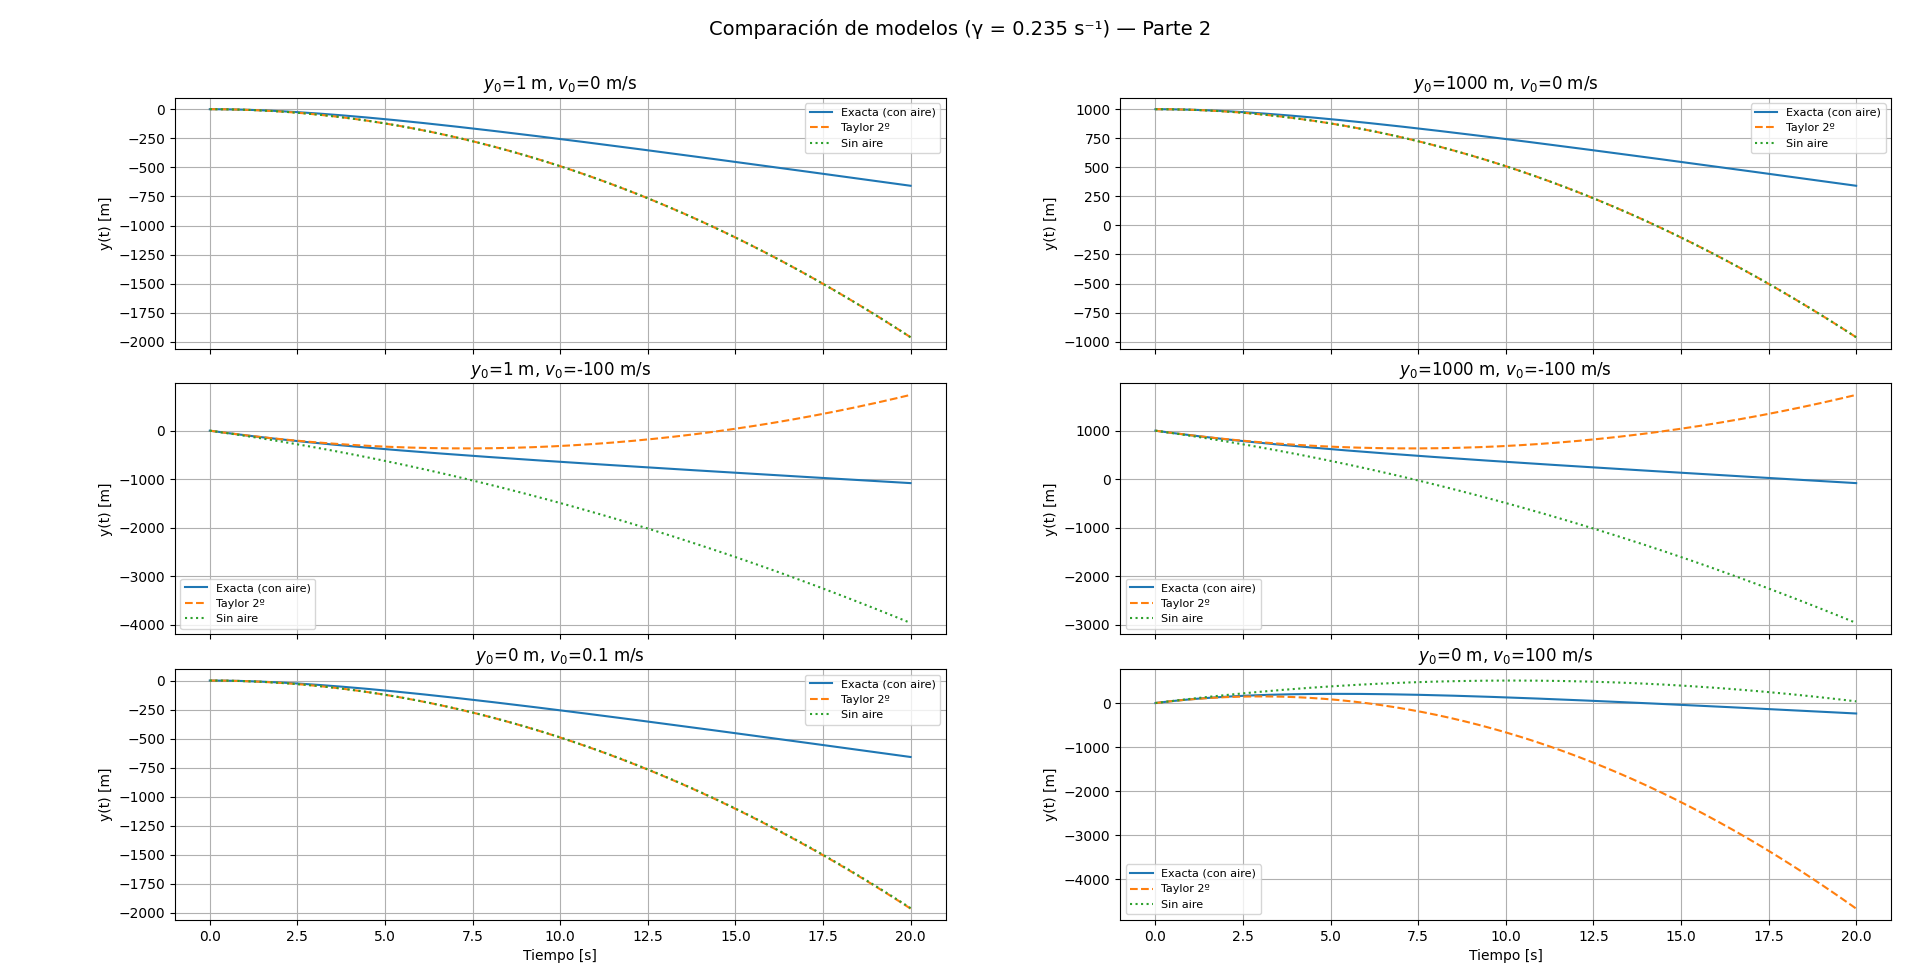
\includegraphics[width=1\textwidth]{assets/comparacion_de_los_modelos_p2.png}
    \caption{Comparación de curvas con distintos valores de $\gamma$}
\end{figure}

\subsubsection{Derivar $y(t)$ y hallar la Velocidad Terminal $v_T$}

Recordando la expresión para el movimiento con rozamiento:

\[
y(t) = y_0 - \frac{g}{\gamma} t - \frac{1}{\gamma} \left( v_0 + \frac{g}{\gamma} \right)\left( e^{-\gamma t} - 1 \right)
\]

Derivando respecto al tiempo:

\[
y'(t) = -\frac{g}{\gamma} + \left( v_0 + \frac{g}{\gamma} \right) e^{-\gamma t}
\]

Tomando el límite cuando $t \to \infty$ se obtiene la velocidad terminal:

\[
v_T = \lim_{t \to \infty} y'(t) = -\frac{g}{\gamma}
\]

Esto indica que la velocidad terminal es constante, negativa (hacia abajo), y de módulo:

\[
|v_T| = \frac{g}{\gamma}
\]

\begin{table}[H]
\centering
\begin{tabular}{|c|c|l|}
\hline
$\gamma$ & $v_T$ (m/s) & Comentario \\
\hline
$\gamma_h = 6.54$ s$^{-1}$ & $-1.50$ & Una hormiga ``planea'' lentamente \\
$\gamma_p = 0.235$ s$^{-1}$ & $-41.7$ & Una persona en caída libre $\approx$ 150 km/h \\
$\gamma_a = 1.05 \cdot 10^{-2}$ s$^{-1}$ & $-933$ & Imposible de alcanzar en la práctica \\
\hline
\end{tabular}
\caption{Velocidades terminales para distintos valores de $\gamma$}
\end{table}

\paragraph{Observaciones:}

\begin{itemize}
    \item Si $v_0 \neq v_T$: la velocidad $y'(t)$ converge exponencialmente a $v_T$ con escala temporal $t_c = \frac{1}{\gamma}$.
    Por ejemplo, para una persona ($\gamma = 0.235$), la velocidad alcanza el 95\% de $v_T$ aproximadamente a los 13 segundos.

    \item Si $v_0 = v_T$: el término $v_0 + \frac{g}{\gamma} = 0$ y desaparece la parte exponencial. En ese caso, $y'(t) = v_T$ para todo $t$, es decir, el cuerpo cae a velocidad constante, describiendo una línea recta.

    \item \textbf{Modelos sin rozamiento}: tanto la caída libre como la aproximación de Taylor ($y_{\text{sr}}$ y $P_2$) no poseen velocidad terminal. En ellos, la velocidad crece linealmente con el tiempo: $y'(t) = v_0 - gt$, y diverge a medida que $t \to \infty$.
\end{itemize}

Para ilustrar el comportamiento de las velocidades terminales, se presenta el siguiente gráfico:
\begin{figure}[H]
    \centering
    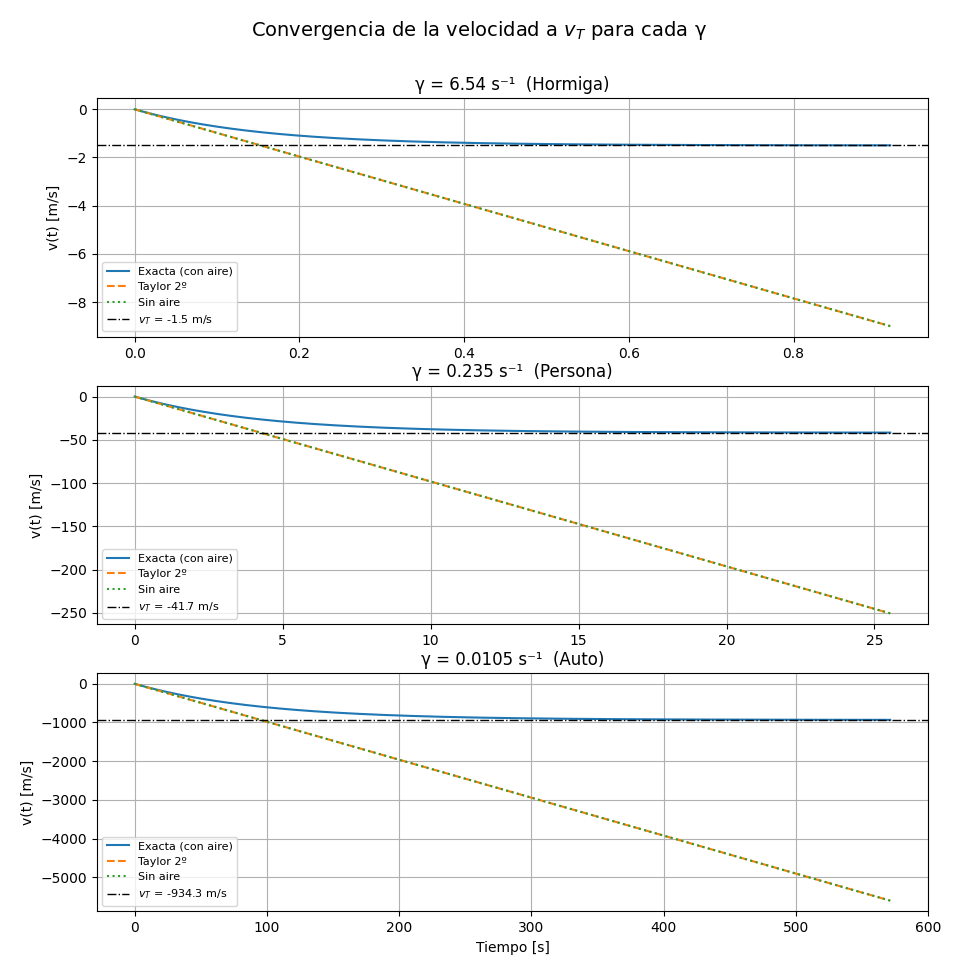
\includegraphics[width=1\textwidth]{assets/comportamiento_VT.png}
    \caption{Velocidades terminales para distintos valores de $\gamma$}
\end{figure}

\paragraph{Comparación de tiempos característicos:}

\begin{itemize}
    \item $\gamma_h$ $\rightarrow t_c = 0.15$ s $\Rightarrow$ alcanza 99\% de $v_T$ en 0.7 s.
    \item $\gamma_p$ $\rightarrow t_c = 4.3$ s $\Rightarrow$ se necesitan $\sim$13 s y $\sim$1000 m para caer a velocidad terminal.
    \item $\gamma_a$ $\rightarrow t_c = 95$ s $\Rightarrow$ aún después de 15 s la velocidad sigue lejos de $v_T$.
\end{itemize}

\subsubsection{¿Cuándo se puede desestimar la resistencia del aire?}

Para el modelo con aire:

\[
y_{\text{roz}}(t) = y_0 + v_0 t - \frac{1}{2}(g + \gamma v_0)t^2 + \mathcal{R}(t^3)
\]

Para el modelo sin aire (caída libre):

\[
y_{\text{libre}}(t) = y_0 + v_0 t - \frac{1}{2}gt^2 + \mathcal{R}(t^3)
\]

Comparando ambos modelos, la diferencia aparece en el término:

\[
\Delta y(t) = \frac{1}{2} \gamma v_0 t^2
\]

Este término cuadrático indica el efecto inicial del rozamiento. Veamos distintos casos:

\begin{table}[H]
\centering
\begin{tabular}{|l|p{10cm}|}
\hline
\textbf{Condición inicial} & \textbf{Rozamiento} \\
\hline
$v_0 = 0$ & La corrección $\frac{1}{2} \gamma v_0 t^2$ desaparece. El efecto del rozamiento es despreciable para $t$ pequeños. Se nota sólo si $\gamma t \gtrsim 1$. \\
\hline
$v_0 = v_T$ & Como $v_0 + \frac{g}{\gamma} = 0$, los modelos con aire y sin aire coinciden hasta orden $t^2$. La resistencia se cancela exactamente. \\
\hline
Lanzamiento fuerte ($v_0 = 100$ m/s) & Para una persona ($\gamma = 0.235$), el término $\frac{1}{2} \gamma v_0 t^2$ es relevante desde $t \approx 4$ s. 
A medida que $t$ crece, el error relativo 
\[
\epsilon(t) = \frac{|\gamma v_0|}{|v_0 - \frac{1}{2}gt|} \cdot t
\]
aumenta, haciendo que el modelo sin rozamiento se vuelva inadecuado. \\
\hline
\end{tabular}
\caption{Cuándo considerar o ignorar el rozamiento del aire}
\end{table}

\subsubsection*{Relación con la masa}

Si $b$ es fijo, se tiene que:

\[
\gamma = \frac{b}{m}, \qquad t_c = \frac{1}{\gamma} = \frac{m}{b}, \qquad \epsilon \propto \gamma \propto \frac{1}{m}
\]

Esto implica que cuanto mayor es la masa del cuerpo, menor es el valor de $\gamma$. Por lo tanto, el término de corrección en el desarrollo de Taylor:

\[
\frac{1}{2} \gamma v_0 t^2
\]

se vuelve insignificante frente al término gravitacional principal $\frac{1}{2}gt^2$. En consecuencia, el movimiento con rozamiento tiende al de caída libre para objetos con gran masa.

\medskip

\textbf{Conclusión:} Un objeto más pesado alcanza el suelo más rápido en presencia de aire debido a que la resistencia tiene menor efecto sobre él.

\medskip

Usando el polinomio de Taylor se observa que se puede despreciar la resistencia del aire cuando:

\[
y(t_{\text{mov}}) \leq 0.3
\]

ya que en este caso el término $\frac{1}{2}\gamma v_0 t^2$ representa aproximadamente un 10\% del valor del término gravitacional $\frac{1}{2}gt^2$, y su impacto es menor.





% --------------------------------------------------------------------
\section{Conclusiones Finales}

A lo largo de este proyecto, exploramos el uso de los \textit{polinomios de Taylor} como una herramienta poderosa para simplificar y comprender fenómenos físicos complejos. Aplicamos esta aproximación matemática a dos situaciones distintas pero muy representativas: la \textbf{variación de la gravedad con la altura} y el \textbf{movimiento de caída con rozamiento del aire}.

En el primer caso, demostramos que, cerca de la superficie terrestre, el valor de la aceleración gravitatoria puede considerarse prácticamente constante. Usando desarrollos de Taylor de orden 1 y 2, mostramos que incluso con diferencias de altura de varios kilómetros (como en el caso del Monte Everest), el error es mínimo. Esto justifica por qué en la mayoría de los problemas cotidianos se utiliza un valor constante para la gravedad.

En el segundo caso, analizamos cómo influye el \textit{rozamiento del aire} en un objeto en caída. Estudiamos diferentes escenarios (velocidades iniciales, masas y constantes de rozamiento) y comparamos los modelos exactos con el modelo sin aire y con su correspondiente polinomio de Taylor de orden 2. Pudimos ver que el \textbf{modelo de Taylor es preciso para tiempos pequeños} o cuando el rozamiento es débil (por ejemplo, en objetos pesados). Sin embargo, cuando se incrementa la velocidad inicial o el tiempo de caída, la diferencia entre modelos se vuelve más notoria.

También se mostró que el desarrollo de Taylor no solo permite simplificar los cálculos, sino que \textbf{ayuda a entender físicamente} en qué condiciones es razonable despreciar ciertos efectos (como el aire) y cuándo no. Por ejemplo, si la corrección debida al rozamiento es menor al 10\% del valor gravitacional, se puede ignorar sin afectar la precisión del resultado.

En definitiva, este trabajo nos permitió ver cómo una técnica matemática aparentemente abstracta puede ser aplicada de forma concreta para tomar decisiones sobre la validez de modelos físicos, estimar errores y encontrar soluciones prácticas en contextos reales. Más allá del cálculo, se trató de \textit{entender mejor el mundo físico desde una mirada matemática fundamentada}.

% --------------------------------------------------------------------
\section{Referencias}
\begin{enumerate}
\item Stewart, J. (2016). \textit{Cálculo de una variable: Trascendentes tempranas} (8ª ed., pp. 774-778). Cengage Learning. $http://www.unet.edu.ve/gilbpar/images/LIBROS/Calculo\ de\ una\ variable\\\ Stewart_9naEd.pdf$
\item LibreTexts. (2020). \textit{Taylor Polynomials} (Sección 8.7). En \textit{Calculus 3e (Apex)}. CC‑BY‑NC 3.0. Recuperado de: $https://math.libretexts.org/Bookshelves/Calculus/Calculus_3e_(Apex)/08\%3\\A_Sequences_and_Series/8.07\%3A_Taylor_Polynomials$
\item S/n. (s.f.). \textit{Taylor} Polinomio de Taylor. Material de la Cátedra de Cálculo Aplicado.

\end{enumerate}

\end{document}